\documentclass[twoside]{book}

% Packages required by doxygen
\usepackage{fixltx2e}
\usepackage{calc}
\usepackage{doxygen}
\usepackage[export]{adjustbox} % also loads graphicx
\usepackage{graphicx}
\usepackage[utf8]{inputenc}
\usepackage{makeidx}
\usepackage{multicol}
\usepackage{multirow}
\PassOptionsToPackage{warn}{textcomp}
\usepackage{textcomp}
\usepackage[nointegrals]{wasysym}
\usepackage[table]{xcolor}

% Font selection
\usepackage[T1]{fontenc}
\usepackage[scaled=.90]{helvet}
\usepackage{courier}
\usepackage{amssymb}
\usepackage{sectsty}
\renewcommand{\familydefault}{\sfdefault}
\allsectionsfont{%
  \fontseries{bc}\selectfont%
  \color{darkgray}%
}
\renewcommand{\DoxyLabelFont}{%
  \fontseries{bc}\selectfont%
  \color{darkgray}%
}
\newcommand{\+}{\discretionary{\mbox{\scriptsize$\hookleftarrow$}}{}{}}

% Page & text layout
\usepackage{geometry}
\geometry{%
  a4paper,%
  top=2.5cm,%
  bottom=2.5cm,%
  left=2.5cm,%
  right=2.5cm%
}
\tolerance=750
\hfuzz=15pt
\hbadness=750
\setlength{\emergencystretch}{15pt}
\setlength{\parindent}{0cm}
\setlength{\parskip}{3ex plus 2ex minus 2ex}
\makeatletter
\renewcommand{\paragraph}{%
  \@startsection{paragraph}{4}{0ex}{-1.0ex}{1.0ex}{%
    \normalfont\normalsize\bfseries\SS@parafont%
  }%
}
\renewcommand{\subparagraph}{%
  \@startsection{subparagraph}{5}{0ex}{-1.0ex}{1.0ex}{%
    \normalfont\normalsize\bfseries\SS@subparafont%
  }%
}
\makeatother

% Headers & footers
\usepackage{fancyhdr}
\pagestyle{fancyplain}
\fancyhead[LE]{\fancyplain{}{\bfseries\thepage}}
\fancyhead[CE]{\fancyplain{}{}}
\fancyhead[RE]{\fancyplain{}{\bfseries\leftmark}}
\fancyhead[LO]{\fancyplain{}{\bfseries\rightmark}}
\fancyhead[CO]{\fancyplain{}{}}
\fancyhead[RO]{\fancyplain{}{\bfseries\thepage}}
\fancyfoot[LE]{\fancyplain{}{}}
\fancyfoot[CE]{\fancyplain{}{}}
\fancyfoot[RE]{\fancyplain{}{\bfseries\scriptsize Generated by Doxygen }}
\fancyfoot[LO]{\fancyplain{}{\bfseries\scriptsize Generated by Doxygen }}
\fancyfoot[CO]{\fancyplain{}{}}
\fancyfoot[RO]{\fancyplain{}{}}
\renewcommand{\footrulewidth}{0.4pt}
\renewcommand{\chaptermark}[1]{%
  \markboth{#1}{}%
}
\renewcommand{\sectionmark}[1]{%
  \markright{\thesection\ #1}%
}

% Indices & bibliography
\usepackage{natbib}
\usepackage[titles]{tocloft}
\setcounter{tocdepth}{3}
\setcounter{secnumdepth}{5}
\makeindex

% Hyperlinks (required, but should be loaded last)
\usepackage{ifpdf}
\ifpdf
  \usepackage[pdftex,pagebackref=true]{hyperref}
\else
  \usepackage[ps2pdf,pagebackref=true]{hyperref}
\fi
\hypersetup{%
  colorlinks=true,%
  linkcolor=blue,%
  citecolor=blue,%
  unicode%
}

% Custom commands
\newcommand{\clearemptydoublepage}{%
  \newpage{\pagestyle{empty}\cleardoublepage}%
}

\usepackage{caption}
\captionsetup{labelsep=space,justification=centering,font={bf},singlelinecheck=off,skip=4pt,position=top}

%===== C O N T E N T S =====

\begin{document}

% Titlepage & ToC
\hypersetup{pageanchor=false,
             bookmarksnumbered=true,
             pdfencoding=unicode
            }
\pagenumbering{alph}
\begin{titlepage}
\vspace*{7cm}
\begin{center}%
{\Large Poligonos \\[1ex]\large 1.\+0 }\\
\vspace*{1cm}
{\large Generated by Doxygen 1.8.14}\\
\end{center}
\end{titlepage}
\clearemptydoublepage
\pagenumbering{roman}
\tableofcontents
\clearemptydoublepage
\pagenumbering{arabic}
\hypersetup{pageanchor=true}

%--- Begin generated contents ---
\chapter{polygons-\/c-\/}
\label{md__r_e_a_d_m_e}
\Hypertarget{md__r_e_a_d_m_e}
\input{md__r_e_a_d_m_e}
\chapter{Hierarchical Index}
\section{Class Hierarchy}
This inheritance list is sorted roughly, but not completely, alphabetically\+:\begin{DoxyCompactList}
\item \contentsline{section}{Point}{\pageref{class_point}}{}
\item \contentsline{section}{Polygon}{\pageref{class_polygon}}{}
\begin{DoxyCompactList}
\item \contentsline{section}{Rectangle}{\pageref{class_rectangle}}{}
\end{DoxyCompactList}
\end{DoxyCompactList}

\chapter{Class Index}
\section{Class List}
Here are the classes, structs, unions and interfaces with brief descriptions\+:\begin{DoxyCompactList}
\item\contentsline{section}{\hyperlink{class_point}{Point} \\*Classe utilizada para representar um ponto em um plano 2D }{\pageref{class_point}}{}
\item\contentsline{section}{\hyperlink{class_polygon}{Polygon} \\*Classe utilizada para representar um polígono em um plano 2D }{\pageref{class_polygon}}{}
\item\contentsline{section}{\hyperlink{class_rectangle}{Rectangle} \\*Classe utilizada para representar um retângulo em um plano 2D }{\pageref{class_rectangle}}{}
\end{DoxyCompactList}

\chapter{Class Documentation}
\hypertarget{class_point}{}\section{Point Class Reference}
\label{class_point}\index{Point@{Point}}


Classe utilizada para representar um ponto em um plano 2D.  




{\ttfamily \#include $<$point.\+h$>$}

\subsection*{Public Member Functions}
\begin{DoxyCompactItemize}
\item 
\hyperlink{class_point_ad92f2337b839a94ce97dcdb439b4325a}{Point} ()
\begin{DoxyCompactList}\small\item\em Construtor padrão. \end{DoxyCompactList}\item 
\hyperlink{class_point_a2bb66002bdd155f2e20ae8e1e55f5c97}{Point} (const float, const float)
\begin{DoxyCompactList}\small\item\em Construtor alternativo. \end{DoxyCompactList}\item 
double \hyperlink{class_point_a8de35a6098cdd7267b4167776da83da6}{getX} ()
\item 
double \hyperlink{class_point_aa278c8bcb8aeb4101023a4baf473b547}{getY} ()
\item 
void \hyperlink{class_point_a61253b28283b54a9cf379132bdff3006}{setX} (float)
\item 
void \hyperlink{class_point_a0a9d3529888cd2fd7c0adb8e46702110}{setY} (float)
\item 
void \hyperlink{class_point_ae456513d2af9dec336514a94e350a386}{set\+XY} (float, float)
\item 
float \hyperlink{class_point_af6595756d7687bf3a324227cbbe2a531}{abs} ()
\item 
float \hyperlink{class_point_a91600d1914ae912e8d9fb9da62feb1bd}{distance} (const \hyperlink{class_point}{Point} \&)
\item 
void \hyperlink{class_point_a2b103de4d519cd01c9864167e12d2c7f}{translate} (const float, const float)
\end{DoxyCompactItemize}
\subsection*{Protected Attributes}
\begin{DoxyCompactItemize}
\item 
double \hyperlink{class_point_ab99c56589bc8ad5fa5071387110a5bc7}{x}
\item 
double \hyperlink{class_point_afa38be143ae800e6ad69ce8ed4df62d8}{y}
\end{DoxyCompactItemize}
\subsection*{Friends}
\begin{DoxyCompactItemize}
\item 
\mbox{\Hypertarget{class_point_a39769dc77d3fa4d361db4ed5822510d6}\label{class_point_a39769dc77d3fa4d361db4ed5822510d6}} 
istream \& {\bfseries operator$>$$>$} (istream \&, \hyperlink{class_point}{Point} \&)
\item 
\mbox{\Hypertarget{class_point_a1a8476a65036945b3fa49c2b6789264e}\label{class_point_a1a8476a65036945b3fa49c2b6789264e}} 
ostream \& {\bfseries operator$<$$<$} (ostream \&, const \hyperlink{class_point}{Point} \&)
\item 
\mbox{\Hypertarget{class_point_a4832a8cf1853edeea25376cb501be7e2}\label{class_point_a4832a8cf1853edeea25376cb501be7e2}} 
bool {\bfseries operator==} (const \hyperlink{class_point}{Point} \&, const \hyperlink{class_point}{Point} \&)
\item 
\mbox{\Hypertarget{class_point_a379ea470d116d5ec7858c3b1c88051fa}\label{class_point_a379ea470d116d5ec7858c3b1c88051fa}} 
\hyperlink{class_point}{Point} {\bfseries operator+} (const \hyperlink{class_point}{Point} \&, const \hyperlink{class_point}{Point} \&)
\item 
\mbox{\Hypertarget{class_point_adc0ae410968ebfcac79ebcf9d4eb3f5b}\label{class_point_adc0ae410968ebfcac79ebcf9d4eb3f5b}} 
\hyperlink{class_point}{Point} {\bfseries operator-\/} (const \hyperlink{class_point}{Point} \&, const \hyperlink{class_point}{Point} \&)
\end{DoxyCompactItemize}


\subsection{Detailed Description}
Classe utilizada para representar um ponto em um plano 2D. 

\begin{DoxyDate}{Date}
Abril, 2017 
\end{DoxyDate}


\subsection{Constructor \& Destructor Documentation}
\mbox{\Hypertarget{class_point_ad92f2337b839a94ce97dcdb439b4325a}\label{class_point_ad92f2337b839a94ce97dcdb439b4325a}} 
\index{Point@{Point}!Point@{Point}}
\index{Point@{Point}!Point@{Point}}
\subsubsection{\texorpdfstring{Point()}{Point()}\hspace{0.1cm}{\footnotesize\ttfamily [1/2]}}
{\footnotesize\ttfamily Point\+::\+Point (\begin{DoxyParamCaption}{ }\end{DoxyParamCaption})}



Construtor padrão. 

Define os valores iniciais de x e y como sendo 0. \mbox{\Hypertarget{class_point_a2bb66002bdd155f2e20ae8e1e55f5c97}\label{class_point_a2bb66002bdd155f2e20ae8e1e55f5c97}} 
\index{Point@{Point}!Point@{Point}}
\index{Point@{Point}!Point@{Point}}
\subsubsection{\texorpdfstring{Point()}{Point()}\hspace{0.1cm}{\footnotesize\ttfamily [2/2]}}
{\footnotesize\ttfamily Point\+::\+Point (\begin{DoxyParamCaption}\item[{const float}]{x,  }\item[{const float}]{y }\end{DoxyParamCaption})}



Construtor alternativo. 

Define os valores iniciais de x e y de acordo com os parâmetros recebidos. 

\subsection{Member Function Documentation}
\mbox{\Hypertarget{class_point_af6595756d7687bf3a324227cbbe2a531}\label{class_point_af6595756d7687bf3a324227cbbe2a531}} 
\index{Point@{Point}!abs@{abs}}
\index{abs@{abs}!Point@{Point}}
\subsubsection{\texorpdfstring{abs()}{abs()}}
{\footnotesize\ttfamily float Point\+::abs (\begin{DoxyParamCaption}{ }\end{DoxyParamCaption})}

Retorna a distância do ponto ao centro do sistema de coordenadas. \mbox{\Hypertarget{class_point_a91600d1914ae912e8d9fb9da62feb1bd}\label{class_point_a91600d1914ae912e8d9fb9da62feb1bd}} 
\index{Point@{Point}!distance@{distance}}
\index{distance@{distance}!Point@{Point}}
\subsubsection{\texorpdfstring{distance()}{distance()}}
{\footnotesize\ttfamily float Point\+::distance (\begin{DoxyParamCaption}\item[{const \hyperlink{class_point}{Point} \&}]{p }\end{DoxyParamCaption})}

Retorna a distância em relação à outro ponto p. \mbox{\Hypertarget{class_point_a8de35a6098cdd7267b4167776da83da6}\label{class_point_a8de35a6098cdd7267b4167776da83da6}} 
\index{Point@{Point}!getX@{getX}}
\index{getX@{getX}!Point@{Point}}
\subsubsection{\texorpdfstring{get\+X()}{getX()}}
{\footnotesize\ttfamily double Point\+::getX (\begin{DoxyParamCaption}{ }\end{DoxyParamCaption})}

Retorna o valor da coordenada x. \mbox{\Hypertarget{class_point_aa278c8bcb8aeb4101023a4baf473b547}\label{class_point_aa278c8bcb8aeb4101023a4baf473b547}} 
\index{Point@{Point}!getY@{getY}}
\index{getY@{getY}!Point@{Point}}
\subsubsection{\texorpdfstring{get\+Y()}{getY()}}
{\footnotesize\ttfamily double Point\+::getY (\begin{DoxyParamCaption}{ }\end{DoxyParamCaption})}

Retorna o valor da coordenada y. \mbox{\Hypertarget{class_point_a61253b28283b54a9cf379132bdff3006}\label{class_point_a61253b28283b54a9cf379132bdff3006}} 
\index{Point@{Point}!setX@{setX}}
\index{setX@{setX}!Point@{Point}}
\subsubsection{\texorpdfstring{set\+X()}{setX()}}
{\footnotesize\ttfamily void Point\+::setX (\begin{DoxyParamCaption}\item[{float}]{x }\end{DoxyParamCaption})}

Define o valor da coordenada x. \mbox{\Hypertarget{class_point_ae456513d2af9dec336514a94e350a386}\label{class_point_ae456513d2af9dec336514a94e350a386}} 
\index{Point@{Point}!set\+XY@{set\+XY}}
\index{set\+XY@{set\+XY}!Point@{Point}}
\subsubsection{\texorpdfstring{set\+X\+Y()}{setXY()}}
{\footnotesize\ttfamily void Point\+::set\+XY (\begin{DoxyParamCaption}\item[{float}]{x,  }\item[{float}]{y }\end{DoxyParamCaption})}

Define o valor das coordenadas x e y. \mbox{\Hypertarget{class_point_a0a9d3529888cd2fd7c0adb8e46702110}\label{class_point_a0a9d3529888cd2fd7c0adb8e46702110}} 
\index{Point@{Point}!setY@{setY}}
\index{setY@{setY}!Point@{Point}}
\subsubsection{\texorpdfstring{set\+Y()}{setY()}}
{\footnotesize\ttfamily void Point\+::setY (\begin{DoxyParamCaption}\item[{float}]{y }\end{DoxyParamCaption})}

Define o valor da coordenada x. \mbox{\Hypertarget{class_point_a2b103de4d519cd01c9864167e12d2c7f}\label{class_point_a2b103de4d519cd01c9864167e12d2c7f}} 
\index{Point@{Point}!translate@{translate}}
\index{translate@{translate}!Point@{Point}}
\subsubsection{\texorpdfstring{translate()}{translate()}}
{\footnotesize\ttfamily void Point\+::translate (\begin{DoxyParamCaption}\item[{const float}]{x,  }\item[{const float}]{y }\end{DoxyParamCaption})}

Translada o ponto em (a,b), sendo a e b números reais (float). 

\subsection{Member Data Documentation}
\mbox{\Hypertarget{class_point_ab99c56589bc8ad5fa5071387110a5bc7}\label{class_point_ab99c56589bc8ad5fa5071387110a5bc7}} 
\index{Point@{Point}!x@{x}}
\index{x@{x}!Point@{Point}}
\subsubsection{\texorpdfstring{x}{x}}
{\footnotesize\ttfamily double Point\+::x\hspace{0.3cm}{\ttfamily [protected]}}

Coordenada x do plano \mbox{\Hypertarget{class_point_afa38be143ae800e6ad69ce8ed4df62d8}\label{class_point_afa38be143ae800e6ad69ce8ed4df62d8}} 
\index{Point@{Point}!y@{y}}
\index{y@{y}!Point@{Point}}
\subsubsection{\texorpdfstring{y}{y}}
{\footnotesize\ttfamily double Point\+::y\hspace{0.3cm}{\ttfamily [protected]}}

Coordenada y do plano 

The documentation for this class was generated from the following files\+:\begin{DoxyCompactItemize}
\item 
Poligonos/point.\+h\item 
Poligonos/point.\+cpp\end{DoxyCompactItemize}

\hypertarget{class_polygon}{}\section{Polygon Class Reference}
\label{class_polygon}\index{Polygon@{Polygon}}


Classe utilizada para representar um polígono em um plano 2D.  




{\ttfamily \#include $<$polygon.\+h$>$}



Inheritance diagram for Polygon\+:\nopagebreak
\begin{figure}[H]
\begin{center}
\leavevmode
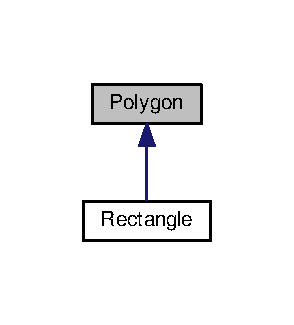
\includegraphics[width=141pt]{class_polygon__inherit__graph}
\end{center}
\end{figure}
\subsection*{Public Member Functions}
\begin{DoxyCompactItemize}
\item 
\hyperlink{class_polygon_af7bc02fdd1541b49aa3f8e2006a30aad}{Polygon} (int)
\begin{DoxyCompactList}\small\item\em Construtor alternativo. \end{DoxyCompactList}\item 
int \hyperlink{class_polygon_a9c28d2deb649781c79a21cee4d884403}{get\+Size} ()
\item 
void \hyperlink{class_polygon_aa7b6a280681bf36afc977f4bd3bcc8d3}{add\+Point} (\hyperlink{class_point}{Point} p)
\begin{DoxyCompactList}\small\item\em Adiciona um objecto Ponto como novo vértice do polígono. \end{DoxyCompactList}\item 
void \hyperlink{class_polygon_a639bed3c0635559f7db23f4fa4e54d89}{add\+Point} (const float, const float)
\item 
void \hyperlink{class_polygon_a5a514d6e28bb6f5e1bccd007e75bb512}{translate} (\hyperlink{class_point}{Point} \&)
\item 
void \hyperlink{class_polygon_ae9ccf7a74ff5ac4dcc776d0e334d9d55}{translate} (const float, const float)
\item 
void \hyperlink{class_polygon_ae56a4c0d4e77bbbe8fa423ca5d33622a}{rotate} (const float, \hyperlink{class_point}{Point})
\item 
double \hyperlink{class_polygon_aaf8aa88f54ac596898c20261f40f77f0}{area} ()
\item 
\hyperlink{class_point}{Point} \hyperlink{class_polygon_a29f2c1c836f16108ea14567728cda0c2}{center} ()
\end{DoxyCompactItemize}
\subsection*{Protected Attributes}
\begin{DoxyCompactItemize}
\item 
const int \hyperlink{class_polygon_ab6ae45da59b24da7c101721dfa784690}{M\+A\+X\+\_\+\+S\+I\+ZE} = 100
\item 
int \hyperlink{class_polygon_aba87c61b99a3812696145bda9e3f466a}{size} = 0
\item 
vector$<$ \hyperlink{class_point}{Point} $>$ \hyperlink{class_polygon_a2d68fb877efd74fd52ea4dea28ea4169}{points}
\end{DoxyCompactItemize}
\subsection*{Friends}
\begin{DoxyCompactItemize}
\item 
\mbox{\Hypertarget{class_polygon_a81a0d6063bf43c894c4a3da261f66c9c}\label{class_polygon_a81a0d6063bf43c894c4a3da261f66c9c}} 
istream \& {\bfseries operator$>$$>$} (istream \&, \hyperlink{class_polygon}{Polygon} \&)
\item 
\mbox{\Hypertarget{class_polygon_a78b2987525d6996d71480891f6402f3d}\label{class_polygon_a78b2987525d6996d71480891f6402f3d}} 
ostream \& {\bfseries operator$<$$<$} (ostream \&, const \hyperlink{class_polygon}{Polygon} \&)
\end{DoxyCompactItemize}


\subsection{Detailed Description}
Classe utilizada para representar um polígono em um plano 2D. 

\begin{DoxyDate}{Date}
Abril, 2017
\end{DoxyDate}
Considere \char`\"{}tamanho\char`\"{} como sendo o número de vértices/pontos do polígono. 

\subsection{Constructor \& Destructor Documentation}
\mbox{\Hypertarget{class_polygon_af7bc02fdd1541b49aa3f8e2006a30aad}\label{class_polygon_af7bc02fdd1541b49aa3f8e2006a30aad}} 
\index{Polygon@{Polygon}!Polygon@{Polygon}}
\index{Polygon@{Polygon}!Polygon@{Polygon}}
\subsubsection{\texorpdfstring{Polygon()}{Polygon()}}
{\footnotesize\ttfamily Polygon\+::\+Polygon (\begin{DoxyParamCaption}\item[{int}]{n }\end{DoxyParamCaption})}



Construtor alternativo. 


\begin{DoxyParams}{Parameters}
{\em n} & Define o tamanho do polígono. \\
\hline
\end{DoxyParams}


\subsection{Member Function Documentation}
\mbox{\Hypertarget{class_polygon_aa7b6a280681bf36afc977f4bd3bcc8d3}\label{class_polygon_aa7b6a280681bf36afc977f4bd3bcc8d3}} 
\index{Polygon@{Polygon}!add\+Point@{add\+Point}}
\index{add\+Point@{add\+Point}!Polygon@{Polygon}}
\subsubsection{\texorpdfstring{add\+Point()}{addPoint()}\hspace{0.1cm}{\footnotesize\ttfamily [1/2]}}
{\footnotesize\ttfamily void Polygon\+::add\+Point (\begin{DoxyParamCaption}\item[{\hyperlink{class_point}{Point}}]{p }\end{DoxyParamCaption})}



Adiciona um objecto Ponto como novo vértice do polígono. 


\begin{DoxyParams}{Parameters}
{\em p} & Ponto a ser adicionado. \\
\hline
\end{DoxyParams}
\mbox{\Hypertarget{class_polygon_a639bed3c0635559f7db23f4fa4e54d89}\label{class_polygon_a639bed3c0635559f7db23f4fa4e54d89}} 
\index{Polygon@{Polygon}!add\+Point@{add\+Point}}
\index{add\+Point@{add\+Point}!Polygon@{Polygon}}
\subsubsection{\texorpdfstring{add\+Point()}{addPoint()}\hspace{0.1cm}{\footnotesize\ttfamily [2/2]}}
{\footnotesize\ttfamily void Polygon\+::add\+Point (\begin{DoxyParamCaption}\item[{const float}]{x,  }\item[{const float}]{y }\end{DoxyParamCaption})}

Cria um objeto Ponto a partir dos paramêtros e o adiciona ao polígono. 
\begin{DoxyParams}{Parameters}
{\em x} & Coordenada x do ponto a ser adicionado. \\
\hline
{\em y} & Coordenada y do ponto a ser adicionado. \\
\hline
\end{DoxyParams}
\begin{DoxySeeAlso}{See also}
\hyperlink{class_polygon_aa7b6a280681bf36afc977f4bd3bcc8d3}{add\+Point(\+Point p)} 
\end{DoxySeeAlso}
\mbox{\Hypertarget{class_polygon_aaf8aa88f54ac596898c20261f40f77f0}\label{class_polygon_aaf8aa88f54ac596898c20261f40f77f0}} 
\index{Polygon@{Polygon}!area@{area}}
\index{area@{area}!Polygon@{Polygon}}
\subsubsection{\texorpdfstring{area()}{area()}}
{\footnotesize\ttfamily double Polygon\+::area (\begin{DoxyParamCaption}{ }\end{DoxyParamCaption})}

Retorna a área do polígono. \mbox{\Hypertarget{class_polygon_a29f2c1c836f16108ea14567728cda0c2}\label{class_polygon_a29f2c1c836f16108ea14567728cda0c2}} 
\index{Polygon@{Polygon}!center@{center}}
\index{center@{center}!Polygon@{Polygon}}
\subsubsection{\texorpdfstring{center()}{center()}}
{\footnotesize\ttfamily \hyperlink{class_point}{Point} Polygon\+::center (\begin{DoxyParamCaption}{ }\end{DoxyParamCaption})}

Retorna um Ponto que representa o centro de massa do polígono. \mbox{\Hypertarget{class_polygon_a9c28d2deb649781c79a21cee4d884403}\label{class_polygon_a9c28d2deb649781c79a21cee4d884403}} 
\index{Polygon@{Polygon}!get\+Size@{get\+Size}}
\index{get\+Size@{get\+Size}!Polygon@{Polygon}}
\subsubsection{\texorpdfstring{get\+Size()}{getSize()}}
{\footnotesize\ttfamily int Polygon\+::get\+Size (\begin{DoxyParamCaption}{ }\end{DoxyParamCaption})}

Retorna o tamanho do polígono. \mbox{\Hypertarget{class_polygon_ae56a4c0d4e77bbbe8fa423ca5d33622a}\label{class_polygon_ae56a4c0d4e77bbbe8fa423ca5d33622a}} 
\index{Polygon@{Polygon}!rotate@{rotate}}
\index{rotate@{rotate}!Polygon@{Polygon}}
\subsubsection{\texorpdfstring{rotate()}{rotate()}}
{\footnotesize\ttfamily void Polygon\+::rotate (\begin{DoxyParamCaption}\item[{const float}]{degrees,  }\item[{\hyperlink{class_point}{Point}}]{p }\end{DoxyParamCaption})}

Rotaciona o polígono em relação à um ponto. 
\begin{DoxyParams}{Parameters}
{\em degrees} & O ângulo ao qual o polígono será rotacionado, em graus. \\
\hline
{\em p} & Ponto de referência.\+de T graus no sentido anti-\/horário em torno de um ponto. \\
\hline
\end{DoxyParams}
\mbox{\Hypertarget{class_polygon_a5a514d6e28bb6f5e1bccd007e75bb512}\label{class_polygon_a5a514d6e28bb6f5e1bccd007e75bb512}} 
\index{Polygon@{Polygon}!translate@{translate}}
\index{translate@{translate}!Polygon@{Polygon}}
\subsubsection{\texorpdfstring{translate()}{translate()}\hspace{0.1cm}{\footnotesize\ttfamily [1/2]}}
{\footnotesize\ttfamily void Polygon\+::translate (\begin{DoxyParamCaption}\item[{\hyperlink{class_point}{Point} \&}]{pt }\end{DoxyParamCaption})}

Translada o polígono para (+x, +y), sendo x e y as coordenadas do parâmetro. \mbox{\Hypertarget{class_polygon_ae9ccf7a74ff5ac4dcc776d0e334d9d55}\label{class_polygon_ae9ccf7a74ff5ac4dcc776d0e334d9d55}} 
\index{Polygon@{Polygon}!translate@{translate}}
\index{translate@{translate}!Polygon@{Polygon}}
\subsubsection{\texorpdfstring{translate()}{translate()}\hspace{0.1cm}{\footnotesize\ttfamily [2/2]}}
{\footnotesize\ttfamily void Polygon\+::translate (\begin{DoxyParamCaption}\item[{const float}]{x,  }\item[{const float}]{y }\end{DoxyParamCaption})}

Translada o polígono para (+x, +y), sendo x e y os parâmetros. 

\subsection{Member Data Documentation}
\mbox{\Hypertarget{class_polygon_ab6ae45da59b24da7c101721dfa784690}\label{class_polygon_ab6ae45da59b24da7c101721dfa784690}} 
\index{Polygon@{Polygon}!M\+A\+X\+\_\+\+S\+I\+ZE@{M\+A\+X\+\_\+\+S\+I\+ZE}}
\index{M\+A\+X\+\_\+\+S\+I\+ZE@{M\+A\+X\+\_\+\+S\+I\+ZE}!Polygon@{Polygon}}
\subsubsection{\texorpdfstring{M\+A\+X\+\_\+\+S\+I\+ZE}{MAX\_SIZE}}
{\footnotesize\ttfamily const int Polygon\+::\+M\+A\+X\+\_\+\+S\+I\+ZE = 100\hspace{0.3cm}{\ttfamily [protected]}}

Número máximo de vértices permitidos. \mbox{\Hypertarget{class_polygon_a2d68fb877efd74fd52ea4dea28ea4169}\label{class_polygon_a2d68fb877efd74fd52ea4dea28ea4169}} 
\index{Polygon@{Polygon}!points@{points}}
\index{points@{points}!Polygon@{Polygon}}
\subsubsection{\texorpdfstring{points}{points}}
{\footnotesize\ttfamily vector$<$\hyperlink{class_point}{Point}$>$ Polygon\+::points\hspace{0.3cm}{\ttfamily [protected]}}

Vetor para guardar os pontos (vértices) do polígono. \mbox{\Hypertarget{class_polygon_aba87c61b99a3812696145bda9e3f466a}\label{class_polygon_aba87c61b99a3812696145bda9e3f466a}} 
\index{Polygon@{Polygon}!size@{size}}
\index{size@{size}!Polygon@{Polygon}}
\subsubsection{\texorpdfstring{size}{size}}
{\footnotesize\ttfamily int Polygon\+::size = 0\hspace{0.3cm}{\ttfamily [protected]}}

Tamanho definido do polígono. 

The documentation for this class was generated from the following files\+:\begin{DoxyCompactItemize}
\item 
Poligonos/polygon.\+h\item 
Poligonos/polygon.\+cpp\end{DoxyCompactItemize}

\hypertarget{class_rectangle}{}\section{Rectangle Class Reference}
\label{class_rectangle}\index{Rectangle@{Rectangle}}


Classe utilizada para representar um retângulo em um plano 2D.  




{\ttfamily \#include $<$rectangle.\+h$>$}



Inheritance diagram for Rectangle\+:\nopagebreak
\begin{figure}[H]
\begin{center}
\leavevmode
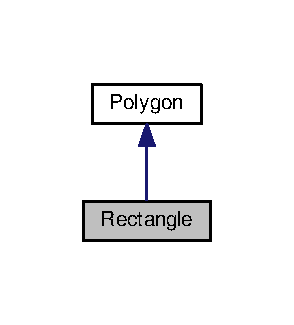
\includegraphics[width=141pt]{class_rectangle__inherit__graph}
\end{center}
\end{figure}


Collaboration diagram for Rectangle\+:\nopagebreak
\begin{figure}[H]
\begin{center}
\leavevmode
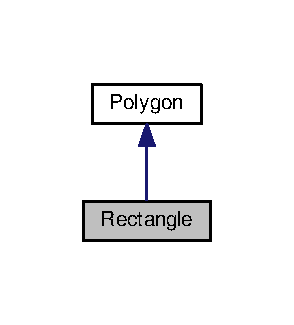
\includegraphics[width=141pt]{class_rectangle__coll__graph}
\end{center}
\end{figure}
\subsection*{Public Member Functions}
\begin{DoxyCompactItemize}
\item 
\hyperlink{class_rectangle_a6772c2d54103b5f097e1c5ac62a87f4e}{Rectangle} (const float x, const float y, const float height, const float width)
\begin{DoxyCompactList}\small\item\em Construtor alternativo. \end{DoxyCompactList}\end{DoxyCompactItemize}
\subsection*{Additional Inherited Members}


\subsection{Detailed Description}
Classe utilizada para representar um retângulo em um plano 2D. 

\begin{DoxyDate}{Date}
Abril, 2017 Esta classe é filha da classe \hyperlink{class_polygon}{Polygon}. 
\end{DoxyDate}


\subsection{Constructor \& Destructor Documentation}
\mbox{\Hypertarget{class_rectangle_a6772c2d54103b5f097e1c5ac62a87f4e}\label{class_rectangle_a6772c2d54103b5f097e1c5ac62a87f4e}} 
\index{Rectangle@{Rectangle}!Rectangle@{Rectangle}}
\index{Rectangle@{Rectangle}!Rectangle@{Rectangle}}
\subsubsection{\texorpdfstring{Rectangle()}{Rectangle()}}
{\footnotesize\ttfamily Rectangle\+::\+Rectangle (\begin{DoxyParamCaption}\item[{const float}]{x,  }\item[{const float}]{y,  }\item[{const float}]{height,  }\item[{const float}]{width }\end{DoxyParamCaption})}



Construtor alternativo. 

Define o tamanho do polígono como sendo 4 (quatro vértices) e sua posição a partir dos parâmetros. 
\begin{DoxyParams}{Parameters}
{\em x} & Posição x do vértice superior esquerdo no plano 2D \\
\hline
{\em y} & Posição y do vértice superior esquerdo no plano 2D \\
\hline
{\em height} & Altura do Retângulo \\
\hline
{\em width} & Largura do Retângulo \\
\hline
\end{DoxyParams}


The documentation for this class was generated from the following files\+:\begin{DoxyCompactItemize}
\item 
Poligonos/rectangle.\+h\item 
Poligonos/rectangle.\+cpp\end{DoxyCompactItemize}

%--- End generated contents ---

% Index
\backmatter
\newpage
\phantomsection
\clearemptydoublepage
\addcontentsline{toc}{chapter}{Index}
\printindex

\end{document}
